\documentclass[a4paper,12pt]{article}

%%% Работа с русским языком

\usepackage{cmap}					% поиск в PDF
\usepackage{mathtext} 				% русские буквы в формулах
\usepackage[T2A]{fontenc}			% кодировка
\usepackage[utf8]{inputenc}			% кодировка исходного текста
\usepackage[english,russian]{babel}	% локализация и переносы
\usepackage{indentfirst}            % красная строка в первом абзаце
\usepackage[unicode]{hyperref}
\usepackage{epigraph}
\frenchspacing                      % равные пробелы между словами и предложениями

%%% Дополнительная работа с математикой
\usepackage{amsmath,amsfonts,amssymb,amsthm,mathtools} % пакеты AMS
\usepackage{bbm} % Blackboard bold для цифр
\usepackage{icomma}                                    % "Умная" запятая

\renewcommand{\phi}{\ensuremath{\varphi}}
\renewcommand{\kappa}{\ensuremath{\varkappa}}
\renewcommand{\le}{\ensuremath{\leqslant}}
\renewcommand{\leq}{\ensuremath{\leqslant}}
\renewcommand{\ge}{\ensuremath{\geqslant}}
\renewcommand{\geq}{\ensuremath{\geqslant}}
\renewcommand{\emptyset}{\ensuremath{\varnothing}}

\newcommand{\cl}{\text{cl }}
\newcommand{\setint}{\text{int }}

\theoremstyle{plain}
\newtheorem{theorem}{Теорема}[section]
\newtheorem{lemma}{Лемма}[section]
\newtheorem{proposition}{Утверждение}[section]
\newtheorem*{corollary}{Следствие}
\newtheorem*{exercise}{Упражнение}

\theoremstyle{definition}
\newtheorem{definition}{Определение}[section]
\newtheorem*{note}{Замечание}
\newtheorem*{reminder}{Напоминание}
\newtheorem*{example}{Пример}
\newtheorem*{tasks}{Вопросы и задачи}

\theoremstyle{remark}
\newtheorem*{solution}{Решение}

%%% Оформление страницы
\usepackage{extsizes}     % Возможность сделать 14-й шрифт
\usepackage{geometry}     % Простой способ задавать поля
\usepackage{setspace}     % Интерлиньяж
\usepackage{enumitem}     % Настройка окружений itemize и enumerate
\setlist{leftmargin=25pt} % Отступы в itemize и enumerate

\geometry{top=25mm}    % Поля сверху страницы
\geometry{bottom=30mm} % Поля снизу страницы
\geometry{left=20mm}   % Поля слева страницы
\geometry{right=20mm}  % Поля справа страницы

\begin{document}
\tableofcontents
\newpage

\section{Теорема Римана об осцилляции}

\begin{definition}
	\textbf{Носителем} функции $f(x)$ называется замыкание множества тех $x$, для которых $f(x) \neq 0$. (supp $f$) Функции с ограниченным носителем называются \textbf{финитными}.
\end{definition}

\begin{definition}
	Множество $D$ называется всюду плотным в множестве $G$, если
	\[\overline{D} = G\]
\end{definition}

\begin{proposition}
	$L_1(\mathbb{R})$ -- линейное нормированное пространство.
	\[\|f\|_1 = \int_\mathbb{R} |f(x)| d\mu(x)\]
\end{proposition}

\begin{lemma}
	Множество непрерывных финитных функций всюду плотно в $L_1(\mathbb{R})$.
\end{lemma}

\begin{proof}
	Заменим $\mathbb{R}$ на $[a,\,b]$. То есть докажем, что множество непрерывных на $[a,\,b]$ функций всюду плотно в $L_1[a,\,b]$.

	\begin{itemize}
		\item Докажем для ограниченных неотрицательных. По теореме о представлении ограниченной измеримой функции пределом последовательности ступенчатых
		      \[\exists \{h_n\}:\: h_n \uparrow f\]
		      Теорема Леви гарантирует, что
		      \[\int_a^n h_n(x)d\mu(x) \to \int_a^b f(x)d\mu(x)\]
		      Значит
		      \begin{align*}
			      \int_a^b |f(x) - h_n(x)|d\mu(x) = \int_a^b (f(x) - h_n(x))d\mu(x) \stackrel{n \to +\infty}{\to} 0
		      \end{align*}
		      То есть нам достаточно доказать, что любую ступенчатую можно приблизить непрерывной:
		      \[h_n(x) = \sum_{k = 1}^N c_k \mathbb{I}_{E_k}(x)\]
		      В силу того, что $\forall k:\: E_k$ -- измеримое, то
		      \[\forall \varepsilon > 0:\: \exists \text{элементарное } M_\varepsilon:\: \mu(E_k \triangle M_\varepsilon) < \varepsilon \]
		      Значит
		      \[\int_a^b |\mathbb{I}_{E_k}(x) - \mathbb{I}_{M_\varepsilon}(x)|d\mu(x) = \int_a^b \mathbb{I}_{E \triangle M_\varepsilon}(x)d\mu(x) = \mu(E \triangle M_\varepsilon) < \varepsilon\]
		      Нам осталось научиться приблизить индикатор интервала непрерывными функциями (так как элементарное множество представимо объединением интервалов), а это сделать очень просто, используя непрерывную функцию $\phi(x)$, которая выглядит вот так:
		      \begin{figure}[h]
			      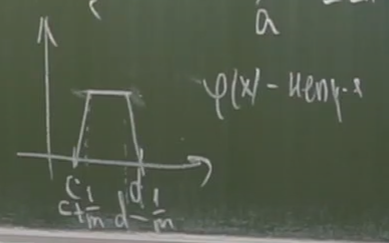
\includegraphics[scale=0.5]{img/phi_graph.png}
			      \caption{Один из способов ввода функции $\phi$}
		      \end{figure}
		      Тогда
		      \[\int_a^b |\mathbb{I}_{(c,\,d)}(x) - \phi(x)|d\mu(x) = \frac{2}{m} < \varepsilon\]
		\item Докажем для любой неотрицательной: как обычно введём срезки, для которых рассуждения аналогичны предыдущему пункту.
		\item Для произвольных расписываем как сумму знакопостоянных.
	\end{itemize}

	Возвращаемся к общему случаю: пусть $f \in L_1(\mathbb{R})$.

	\[\exists N \in \mathbb{N}\: \int_{\mathbb{R} \setminus [-N,\,N]}|f(x)|d\mu(x) < \frac{\varepsilon}{3}\]
	По доказанному выше:
	\[f|_{[-N,\,N]} :\: \forall \varepsilon > 0 \:\exists g \in C[-N,\,N] \: \|f|_{[-N,\,N]} - g\|_{L_1[-N,\,N]} < \frac{\varepsilon}{3}\]
	Далее мы можем продлить $g$ на всю прямую линейных образом (аналогично введению функции $\phi$ из рассуждений выше), так, чтобы
	\[\int_{\mathbb{R}\setminus [-N,\,N]} |g(x)|d\mu(x) < \frac{\varepsilon}{3}\]
	Тогда
	\[\int_\mathbb{R} |f(x) - g(x)|d\mu(x) \leq \int_{-N}^N |f(x) - g(x)|d\mu(x) + \int_{\mathbb{R} \setminus [-N,\,N]} (|f(x)| + |g(x)|) d\mu(x) < \varepsilon\]
\end{proof}

\begin{lemma}
	Каждая суммируемая на $\mathbb{R}$ функция $f(x)$ непрерывна в среднем относительно сдвига, то есть
	\[\lim_{t \to 0} \int_\mathbb{R} |f(x + t) - f(x)| d\mu(x) = 0\]
\end{lemma}

\begin{proof}
	Докажем, что для $f \in L_1[a,\,b]$:
	\[\lim_{\delta \to +0} \sup_{0 \leq h \leq \delta} \int_a^{b - h} |f(x + h) - f(x)|d\mu(x) = 0\]
	По предыдущей лемме:
	\[\forall \varepsilon > 0 \: \exists g \in C[a,\,b]:\: \int_a^b |f(x) - g(x)|d\mu(x) < \frac{\varepsilon}{3}\]
	$g$ -- непрерывная на $[a,\,b] \Rightarrow$ по теореме Кантора:
	\[\forall \varepsilon > 0 \: \exists \delta > 0 \: \forall x,\,y \in [a,\,b],\, |x - y| < \delta :\: |g(x) - g(y)| < \frac{\varepsilon}{3(b - a)}\]
	Тогда $\forall h \: 0 \leq h \leq \delta$:
	\begin{align*}
		\int_a^{b - h}|f(x + h) - f(x)|d\mu(x) \leq \int_a^{b - h} |f(x + h) - g(x + h)|d\mu(x) + \int_a^{b - h}|f(x) - g(x)|d\mu(x) + \\
		+ \int_a^{b - h}|g(x + h) - g(x)|d\mu(x) < \varepsilon
	\end{align*}
	Так как $f$ суммируема на $\mathbb{R}$, то $\exists N \in \mathbb{N}$:
	\[\int_{\mathbb{R} \setminus [-N,\,N]}|f(x)|d\mu(x) < \frac{\varepsilon}{3}\]
	Тогда выберем $[a,\,b] := [-N - 1,\,N + 1]$ и введём $g := f\mathbb{I}_{[-N,\,N]} \in L_1[a,\,b]$. Применим к этой функции доказанное выше равенство:
	\[\exists \delta \in (0,\,1) \: \forall h,\, 0 \leq h \leq \delta :\: \int_a^{b - h}|g(x + h) - g(x)|d\mu(x) < \frac{\varepsilon}{3}\]
	Теперь возьмём $\forall t,\, |t| < \delta$:
	\[
		\int_\mathbb{R}|f(x + t) - f(x)|d\mu(x) = \int\limits_{\{x,\,x+t\}\subseteq[a,\,b]}|f(x+t)-f(x)|d\mu(x) + \int\limits_{\{x,\,x+y\}\not\subseteq[a,\,b]}|f(x+t)-f(x)|d\mu(x) < \varepsilon
	\]
\end{proof}

\begin{theorem}
	Римана об осцилляции.

	Если $f \in L_1(I)$, где $I$ -- конечный или бесконечный промежуток, то
	\[\lim_{\lambda \to \infty} \int_I f(x)\cos(\lambda x) d \mu(x) = \lim_{\lambda \to \infty} \int_I f(x) \sin (\lambda x) d\mu(x) = 0\]
\end{theorem}

\begin{proof}
	\begin{align*}
		\int_I f(x) \cos(\lambda x) d\mu(x) \stackrel{x = t + \frac{\pi}{\lambda}}{=} - \int_{I - \frac{\pi}{\lambda}} f\left( t + \frac{\pi}{\lambda} \right) \cos(\lambda t) d \mu(t) = \\
		-\frac{1}{2} \int_I \left(f\left(t + \frac{\pi}{\lambda}\right) - f(t) \right)\cos(\lambda t) d\mu(t) - \frac{1}{2} \int_{(I - \frac{\pi}{\lambda}) \triangle I} f\left(t + \frac{\pi}{\lambda}\right) \cos(\lambda t) d \mu(t)
	\end{align*}
	Заметим, что
	\begin{align*}
		\left|\int_{(I - \frac{\pi}{\lambda}) \setminus I} f\left(t + \frac{\pi}{\lambda}\right) \cos(\lambda t) d \mu(t)\right| \leq \int_{(I - \frac{\pi}{\lambda}) \triangle I} \left|f\left(t + \frac{\pi}{\lambda}\right)\right| d\mu(t) = \\
		= \int_{I \triangle (I + \frac{\pi}{\lambda})} |f(x)|d\mu(t) \stackrel{\lambda \to \infty}{\to} 0
	\end{align*}
	Последнее заключение следует из того, что $\mu\left(I \triangle (I + \frac{\pi}{\lambda})\right) \stackrel{\lambda \to \infty}{\to} 0$

	Также очевидно, что
	\begin{align*}
		\left|\int_I \left(f\left(t + \frac{\pi}{\lambda}\right) - f(t) \right)\cos(\lambda t) d\mu(t)\right| \leq \int_I \left|f\left(t + \frac{\pi}{\lambda}\right) - f(t)\right|d\mu(t) \stackrel{\text{по пред. Лемме}}{\to} 0
	\end{align*}
\end{proof}

\end{document}
